\documentclass[tikz]{standalone}
\begin{document}

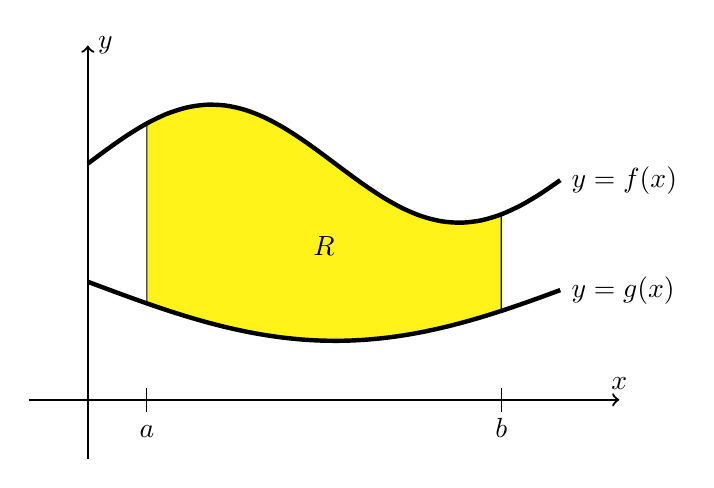
\begin{tikzpicture}[scale=1.5]
      
  % shade region
  \draw[smooth,fill=yellow!90] plot[domain=0.5:3.5] ({\x},{2 + 0.5*sin(1.5*\x r)}) --
  plot[domain=3.5:0.5] ({\x},{1 - 0.5*sin(0.75*\x r)}) -- cycle;

  % draw axes
  \draw[thick,->] (-0.5,0) -- (4.5,0) node[above] {$x$};
  \draw[thick,->] (0,-0.5) -- (0,3) node[right] {$y$};

  % draw curve
  \draw[ultra thick,domain=0:4,smooth] plot ({\x},{2 + 0.5*sin(1.5*\x r)}) node[right] {$y=f(x)$};
  \draw[ultra thick,domain=0:4,smooth] plot ({\x},{1 - 0.5*sin(0.75*\x r)}) node[right] {$y=g(x)$};

  \draw (0.5,0.1) -- (0.5,-0.1);
  \draw (0.5,-0.4) node[above] {$a$};
  \draw (3.5,0.1) -- (3.5,-0.1);
  \draw (3.5,-0.4) node[above] {$b$};

  \node at (2,1.3) {$R$};
    
\end{tikzpicture}
\end{document} 



```{admonition} Computing the Area between Two Curves
:class: info

Suppose $f$ and $g$ are continuous functions with $f(x) \geq g(x)$ on $[a,b]$.

Then the area of the region, $R$, bounded above by $y=f(x)$ and below by $y=g(x)$ on $[a,b]$ is given by

$$\int_a^b f(x)-g(x) ~dx.$$
